\chapter[APÊNDICE \ref{Ap:Cavity}]{Cavidade bidimensional}
\label{Ap:Cavity}

Um problema comumente utilizado na literatura como \textit{benchmark}, trata-se de uma cavidade quadrada ($\Omega=[-1,1]^2$) com paredes aderentes, onde o fluido encontra-se confinado e sujeito a uma velocidade prescrita $\BB{u}_\infty$ ocasionada devido ao deslizamento de uma parede na face superior da cavidade. Nesse sentido são observados os efeitos provocados no fluido devido à diferentes números de Reynolds, o qual é calculado por meio da equação \ref{eq:Reynolds}:

\begin{equation}
    \Rey=\frac{\rho L\norm{\BB{u}_\infty}}{\mu}\text{,}
    \label{eq:Reynolds}
\end{equation}

\noindent em que $L$ é o comprimento característico, que no caso analisado é igual ao lado da cavidade. Dessa forma considera-se uma velocidade constante para todas as análises de $\BB{u}_\infty=\{1,0\}^T$, sendo os diferentes números de Reynolds obtidos pela variação da viscosidade do fluido. A Figura \ref{fig:cavity} apresenta esquematicamente o problema simulado.

\begin{figure}[h!]
    \centering
    \caption{Desenho esquemático do problema de cavidade.}
    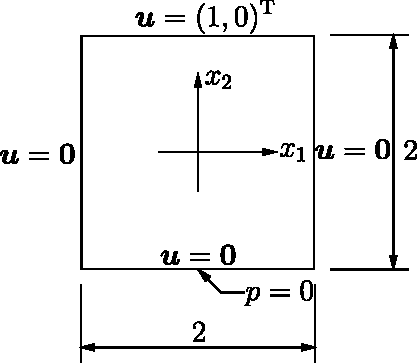
\includegraphics[width=.35\linewidth]{Figuras/Cavity/cavidade.pdf}
    \\Fonte: Autoria Própria (\the\year).
    \label{fig:cavity}
\end{figure}

Pelo fato do problema possuir apenas fronteiras do tipo Dirichlet, o condicionamento da solução do campo de pressões é garantido pela aplicação de uma condição de pressão nula no vértice superior direito da cavidade, conforme visto na figura acima.  Também se observa que existe uma descontinuidade nas condições de contorno no encontro entre as paredes da cavidade e seu topo, podendo ser consideradas velocidades nulas ou igual à velocidade do topo. No problema em questão considerou-se que a velocidade nesse ponto é igual à $\BB{u}_\infty$.

A malha de elementos finitos foi feita pela subdivisão do domínio em 20000 elementos dispostos de maneira estruturada com orientação à esquerda, conforme observado na Figura \ref{fig:cavity_disc}. O número de graus de liberdade para a simulação VMS de aproximação linear, quadrática e LES são 30603, 121203 e 91003, respectivamente. Os parâmetros utilizados foram $\rho=1$ para todas as análises, $\mu=0,02$, $\mu=5\times10^{-3}$, $\mu=2\times10^{-3}$, $\mu=4\times10^{-4}$, $\mu=2,6667\times10^{-4}$ e $\mu=2\times10^{-4}$, resultando em $\Rey=100$, $\Rey=400$, $\Rey=1000$, $\Rey=5000$, $\Rey=7500$ e $\Rey=10000$, respectivamente. Os modelos utilizados foram o VMS com aproximação linear e quadrática e o LES com elementos de Taylor-Hood P2P1 e $C_S=0,10$. O passo de tempo em todos os casos foi de $\Delta t=0,1$ e a simulação foi mantida até que a estacionariedade dos parâmetros do fluxo fosse alcançada.

\begin{figure}[h!]
    \centering
    \caption{Malha considerada para o problema de cavidade.}
    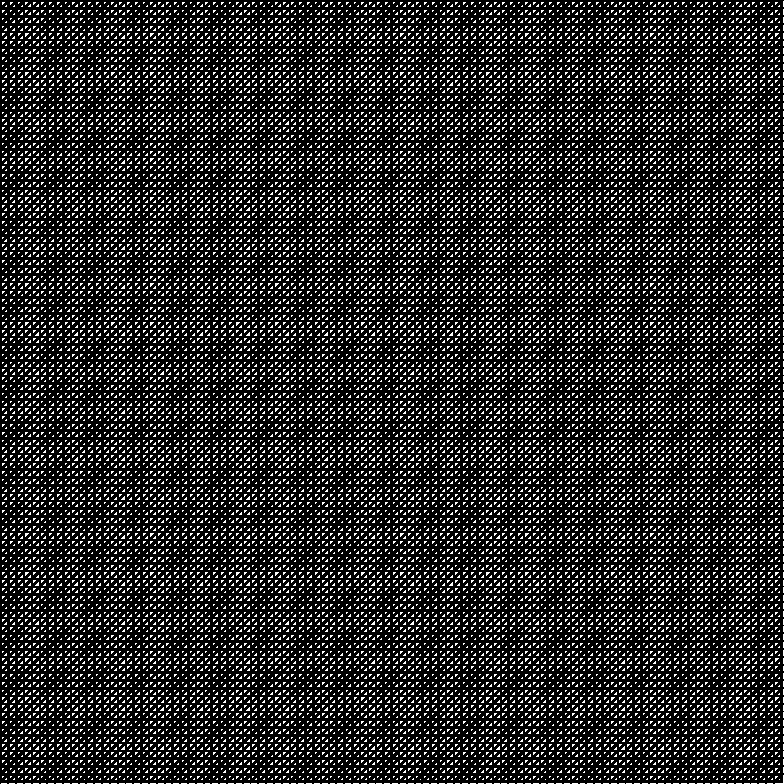
\includegraphics[width=.6\linewidth]{Figuras/Cavity/mesh.pdf}
    \\Fonte: Autoria Própria (\the\year).
    \label{fig:cavity_disc}
\end{figure}

Como o problema apresenta características de um escoamento quase-estático, a parcela dos termos inerciais foram desprezados em ambos os modelos de turbulência. Além disso, os resultados adquiridos para um determinado número de Reynolds foram aplicados como valores iniciais para a determinação dos resultados para a próxima análise.

Os resultados obtidos foram comparados com aqueles apresentados por \citeonline{ghia1982high}. A Figura \ref{fig:cavity-results} apresenta os valores do campo de velocidades sobre as linhas médias da cavidade ($x_1=0$ e $x_2=0$).

\begin{figure}[h!]
    \centering
    \caption{Valores do campo de velocidades sobre as linhas médias da cavidade.}
    \begin{subfigure}{0.4\textwidth}
        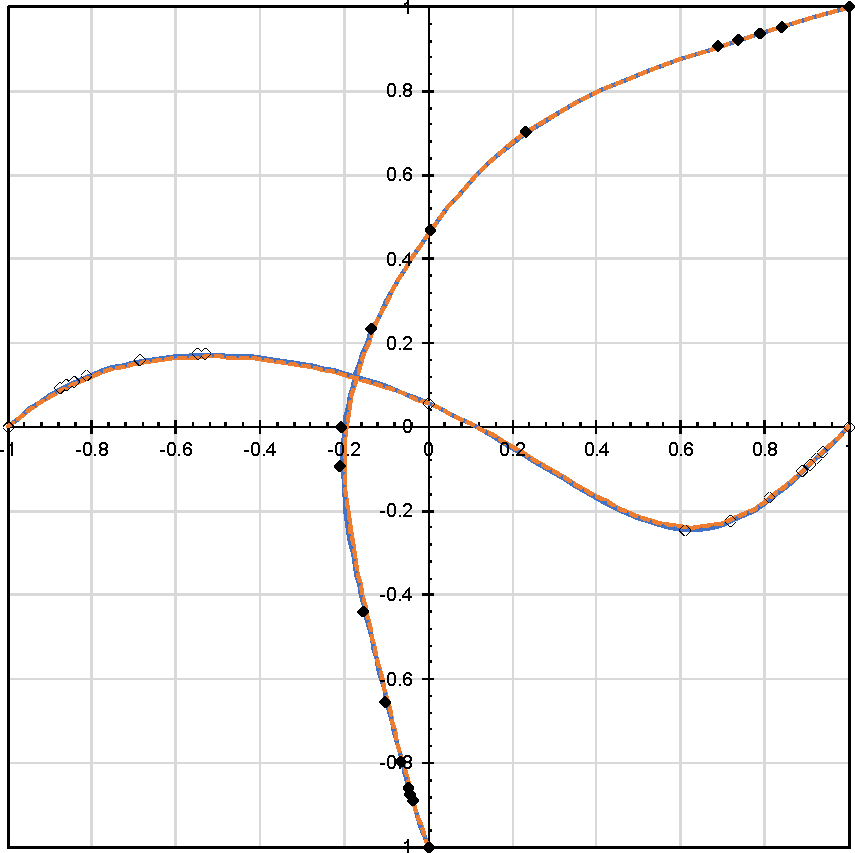
\includegraphics[width=\linewidth]{Figuras/Cavity/Re100.pdf}
        \caption{$\Rey=100$}
    \end{subfigure}
    \begin{subfigure}{0.4\textwidth}
        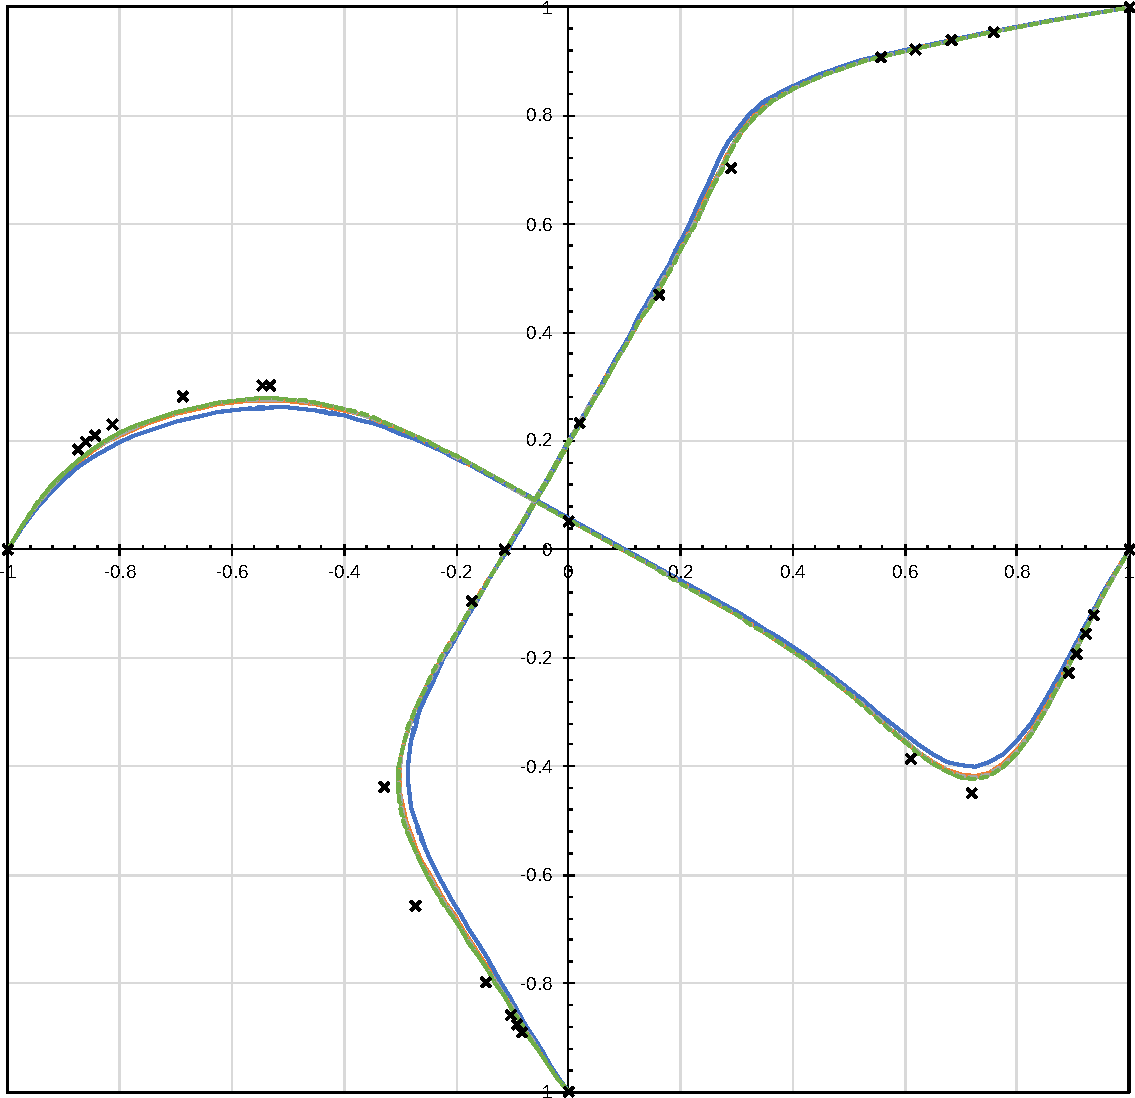
\includegraphics[width=\linewidth]{Figuras/Cavity/Re400.pdf}
        \caption{$\Rey=400$}
    \end{subfigure}
    \begin{subfigure}{0.4\textwidth}
        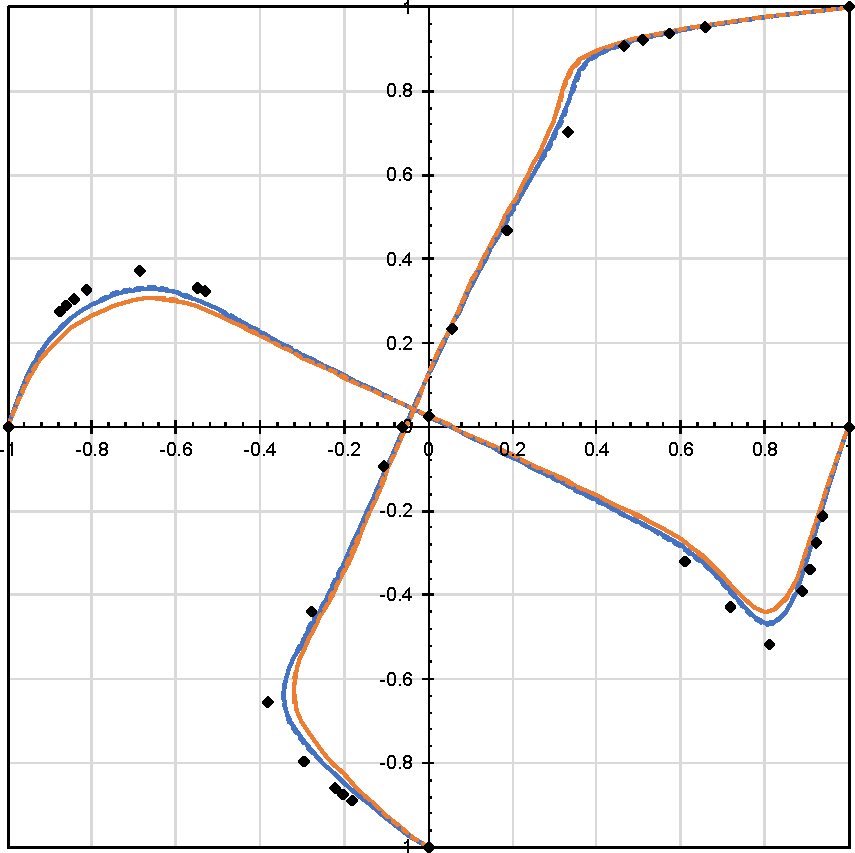
\includegraphics[width=\linewidth]{Figuras/Cavity/Re1000.pdf}
        \caption{$\Rey=1000$}
    \end{subfigure}
    \begin{subfigure}{0.4\textwidth}
        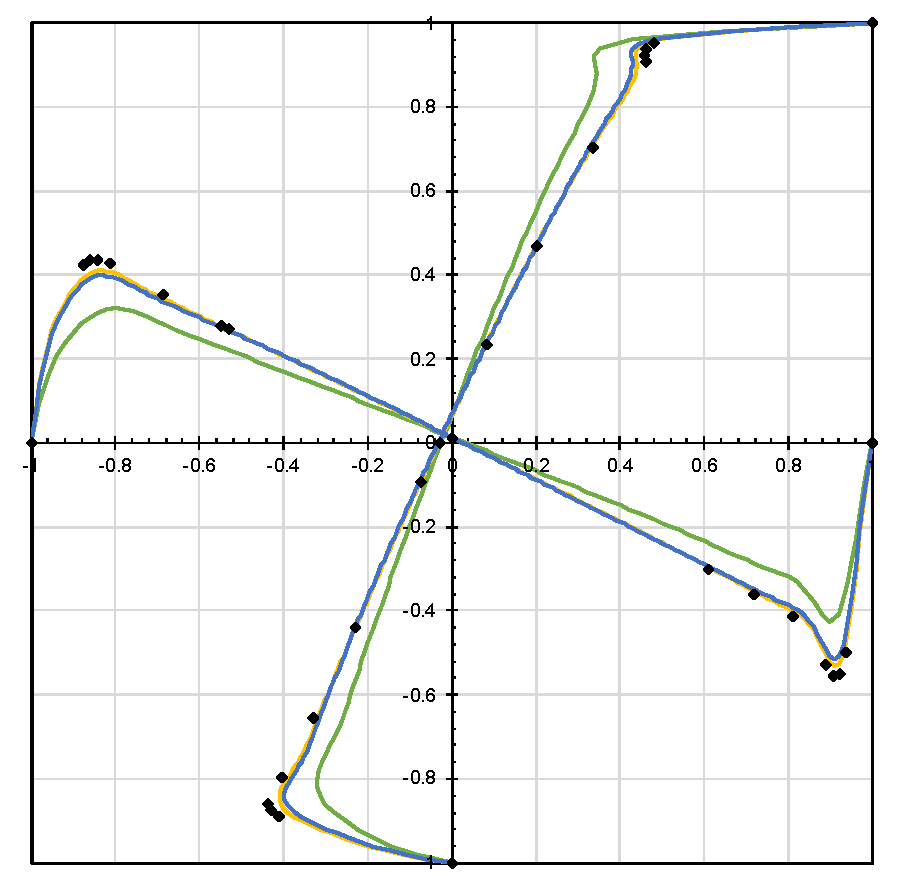
\includegraphics[width=\linewidth]{Figuras/Cavity/Re5000.pdf}
        \caption{$\Rey=5000$}
    \end{subfigure}
    \begin{subfigure}{0.4\textwidth}
        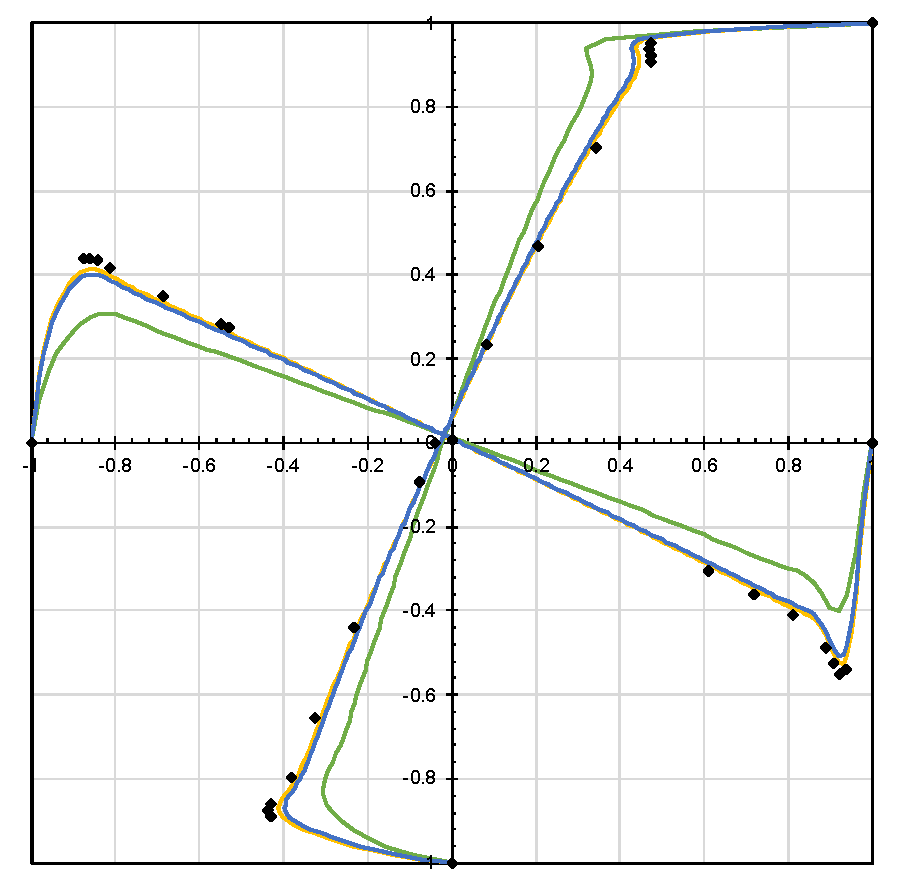
\includegraphics[width=\linewidth]{Figuras/Cavity/Re7500.pdf}
        \caption{$\Rey=7500$}
    \end{subfigure}
    \begin{subfigure}{0.4\textwidth}
        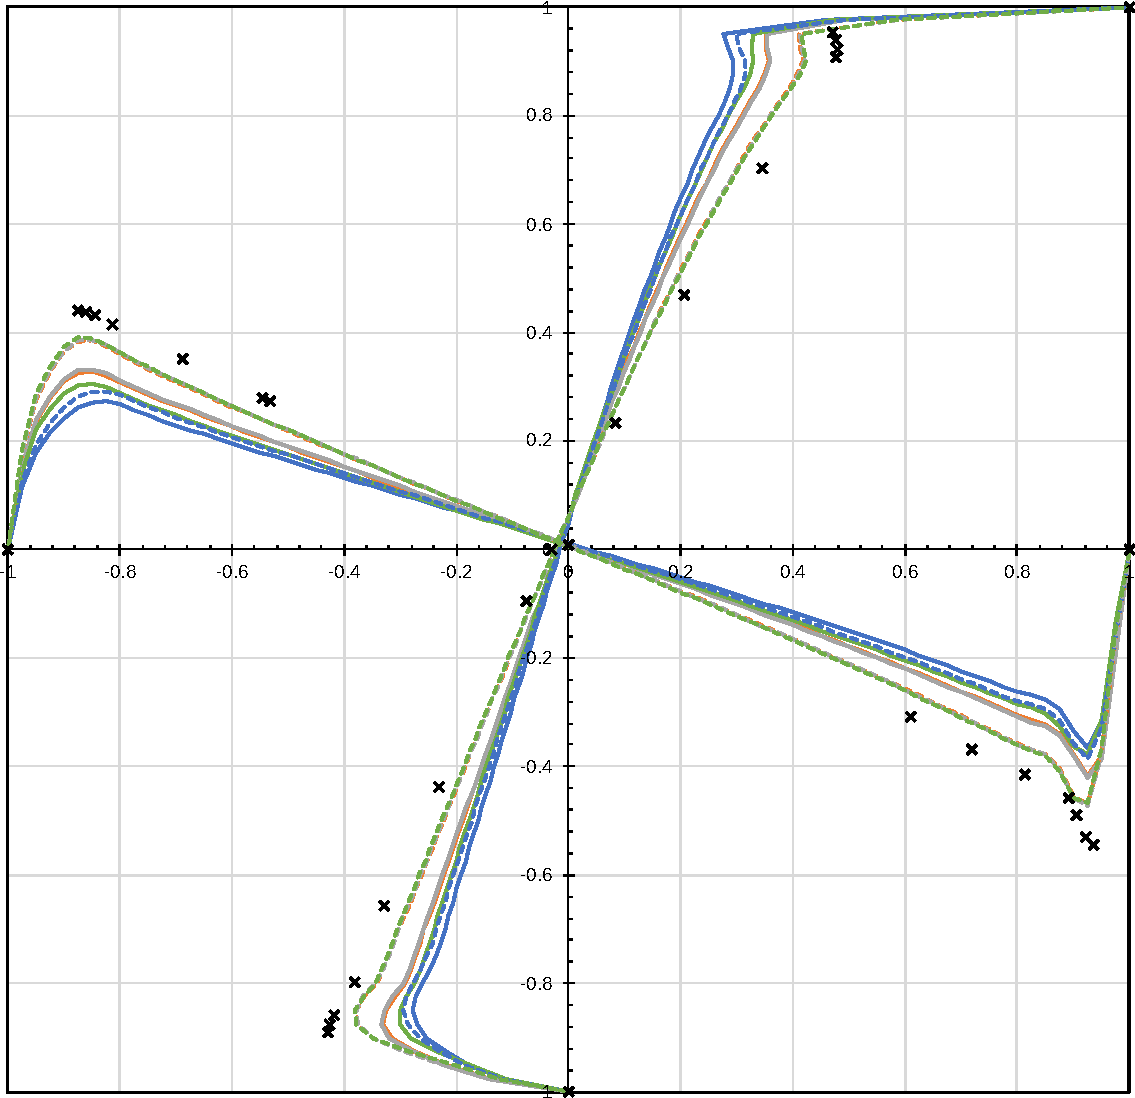
\includegraphics[width=\linewidth]{Figuras/Cavity/Re10000.pdf}
        \caption{$\Rey=10000$}
    \end{subfigure}
    \begin{subfigure}{\textwidth}
        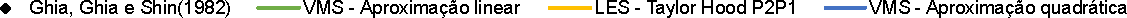
\includegraphics[width=\linewidth]{Figuras/Cavity/Legenda.pdf}
    \end{subfigure}
    \\Fonte: Autoria Própria (\the\year).
    \label{fig:cavity-results}
\end{figure}

A Figura \ref{fig:cavity-results2} apresenta o campo de velocidades na cavidade após o escoamento atingir seu estado estacionário.

\begin{figure}[h!]
    \centering
    \caption{Campo de velocidades em regime estacionário na cavidade.}
    \begin{subfigure}{0.32\textwidth}
        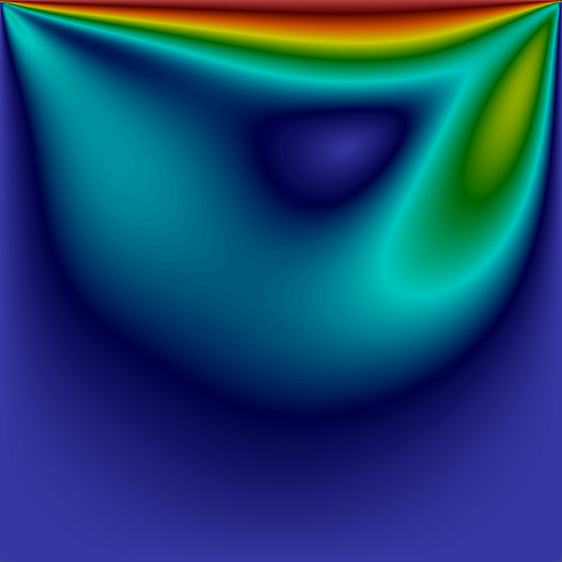
\includegraphics[width=\linewidth]{Figuras/Cavity/Re100.png}
        \caption{$\Rey=100$}
    \end{subfigure}
    \begin{subfigure}{0.32\textwidth}
        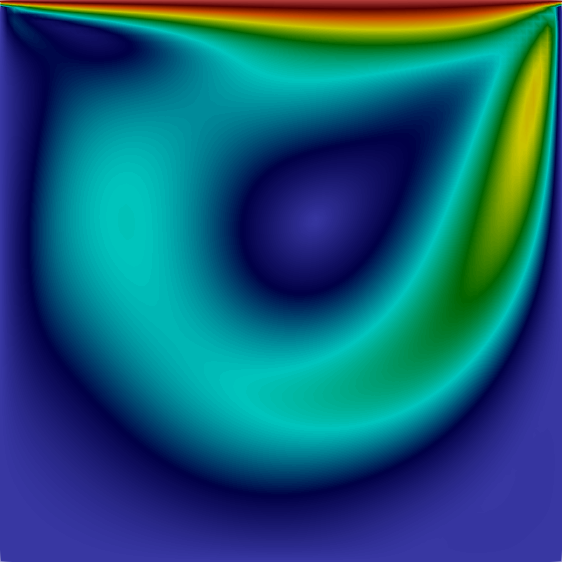
\includegraphics[width=\linewidth]{Figuras/Cavity/Re400.png}
        \caption{$\Rey=400$}
    \end{subfigure}
    \begin{subfigure}{0.32\textwidth}
        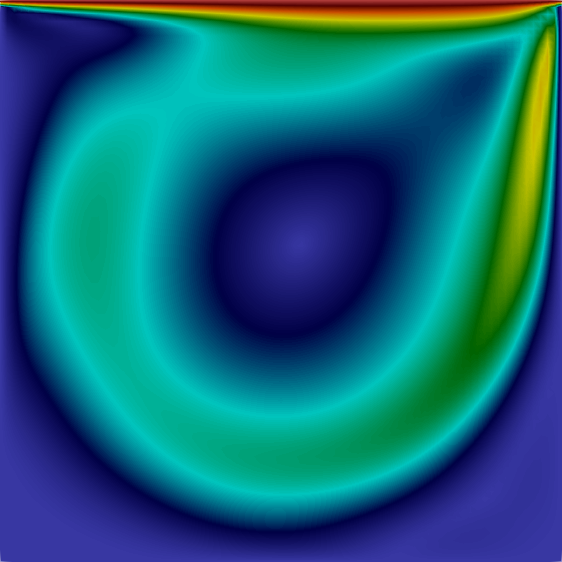
\includegraphics[width=\linewidth]{Figuras/Cavity/Re1000.png}
        \caption{$\Rey=1000$}
    \end{subfigure}
    \begin{subfigure}{0.32\textwidth}
        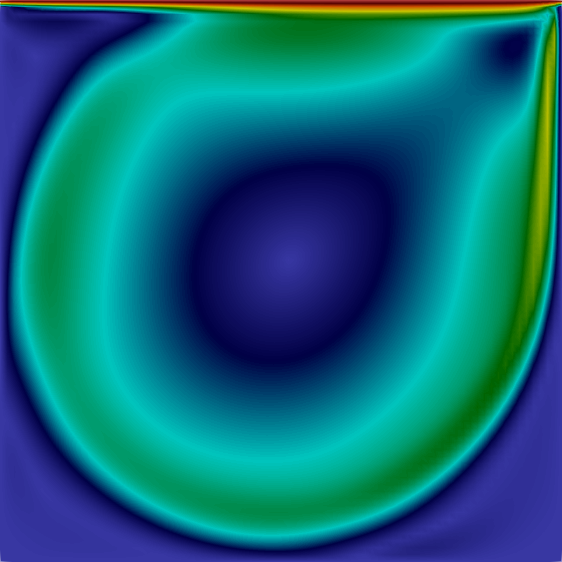
\includegraphics[width=\linewidth]{Figuras/Cavity/Re5000.png}
        \caption{$\Rey=5000$}
    \end{subfigure}
    \begin{subfigure}{0.32\textwidth}
        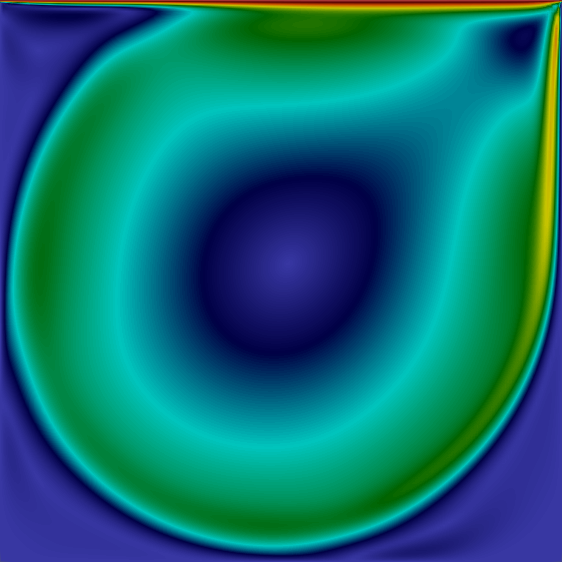
\includegraphics[width=\linewidth]{Figuras/Cavity/Re7500.png}
        \caption{$\Rey=7500$}
    \end{subfigure}
    \begin{subfigure}{0.32\textwidth}
        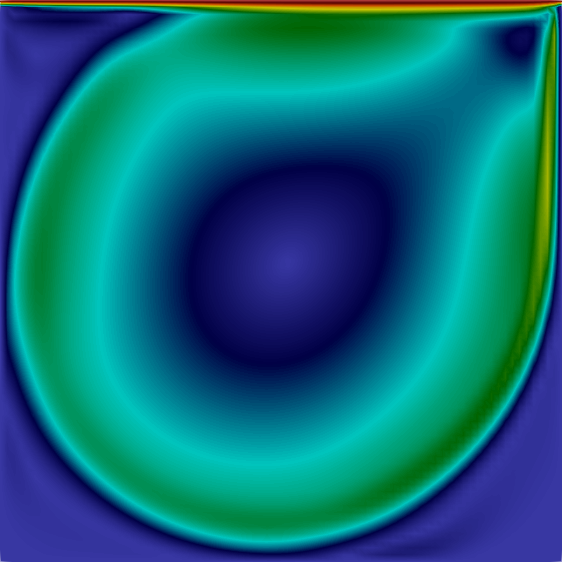
\includegraphics[width=\linewidth]{Figuras/Cavity/Re10000.png}
        \caption{$\Rey=10000$}
    \end{subfigure}
    \begin{subfigure}{0.4\textwidth}
        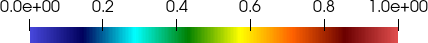
\includegraphics[width=\linewidth]{Figuras/Cavity/Legenda.png}
    \end{subfigure}
    \\Fonte: Autoria Própria (\the\year).
    \label{fig:cavity-results2}
\end{figure}

Para todas as simulações conduzidas, percebeu-se que houve uma excelente concordância dos resultados para números de Reynolds baixos, no entanto a simulação VMS de aproximação linear passou a apresentar resultados cada vez mais discrepantes à medida que o número de Reynolds aumentou, enquanto o VMS de aproximação quadrática e o LES apresentaram resultados mais próximos aos de \citeonline{ghia1982high}, sendo que o LES apresentou resultados ligeiramente melhores em relação ao VMS quadrático. Para número de Reynolds muito altos observou-se um leve desvio nos resultados próximos à parede superior da cavidade, o que poderia ser melhorado caso uma discretização mais fina da malha fosse empregada nessa região.